% !TeX program = xelatex
\documentclass[9pt]{beamer}
\usepackage{xcolor}
\definecolor{orange}{HTML}{71697A}
\definecolor{lightgray}{HTML}{CCCCCC}
\definecolor{red}{HTML}{AC454A}
\definecolor{brown}{HTML}{EAD296}
\definecolor{darkgrey}{HTML}{313630}
\definecolor{cornflower}{HTML}{247BA0}
\definecolor{sienna}{HTML}{6C464F}
\usefonttheme{professionalfonts} % using non standard fonts for beamer
\usefonttheme{serif} % default family is serif
\usepackage{fontspec}
\usepackage{setspace}
\usepackage{natbib}
\usepackage{animate}
\usepackage{graphicx}
%\usepackage[T1]{fontenc}

\bibliographystyle{abbrv}
%\setmainfont{Liberation Serif}
%\setmainfont{Liberation Serif}
\setmainfont{Comfortaa}
%\usepackage[T1]{fontenc}

\setbeamercolor{frametitle}{bg=orange,fg=white}
\setbeamercolor{author in head/foot}{bg=orange,fg=white}

%\setbeamerfont{page number}{size=\Huge}

%\setbeamertemplate{itemize itemjpegs}[circle]
\useinnertheme{circles}
\setbeamercolor{palette primary}{bg=orange,fg=white}
%\setbeamercolor{palette secondary}{bg=red,fg=white}
\setbeamertemplate{itemize item}{\color{darkgrey}$\circ$}
\setbeamercolor{structure}{fg=darkgrey} % itemize, enumerate, etc

%\setbeamercolor{section in head/foot}{bg=red}
\setbeamercolor{title}{fg=orange} %, bg=brown
\setbeamercolor{author}{fg=darkgrey}
\setbeamercolor{institute}{fg=darkgrey}
\setbeamercolor{date}{fg=darkgrey}
%\setbeamercolor{normal text}{fg=darkgrey}
\makeatletter
\setbeamertemplate{headline}{%
	\usebeamercolor[bg]{frametitle}\rule{\textwidth}{1cm}
}
\setbeamerfont{title}{size=\LARGE}
\setbeamerfont{institute}{size=\normalsize}
\renewcommand*{\bibfont}{\scriptsize}


\setbeamertemplate{frametitle}{%
	\vskip-1cm%
	\begin{minipage}[c][\headheight][c]{\textwidth}%
		\usebeamerfont{frametitle}
		\strut\insertframetitle\par
		{%
			\ifx\insertframesubtitle\@empty%
			\else%
			{\usebeamerfont{framesubtitle}\usebeamercolor[fg]{framesubtitle}\strut\insertframesubtitle\par}%
			\fi
		}%      
		\vspace*{0.05cm}
	\end{minipage}%
	\vskip-0.1em
}
%\setbeamertemplate{footline}{%
%	\leavevmode%
%	\hbox{\begin{beamercolorbox}[wd=\paperwidth,ht=4.5ex,dp=3.125ex]{author in head/foot}%
%			\usebeamerfont{author in head/foot} bar
%	\end{beamercolorbox}}%
%	\vskip0pt%
%}
\makeatother


\title{The Interactive Isnalyser \\
	\small Making Transmissions of Oral Tradition Tangible}
\author{Maroussia Bednarkiewicz and Stefan Wezel}
\institute{mlcolab @ Tübingen University Cluster of Excellence}

\date{\today}


%\setbeamertemplate{sidebar right}{}
%\setbeamertemplate{footline}{%
%	\hfill\usebeamertemplate***{navigation symbols}
%	\hspace{1cm}\insertframenumber{}}
\setbeamerfont{page number in head/foot}{size=\small}
    \setbeamertemplate{footline}{%
	\raisebox{5pt}{\makebox[\paperwidth]{\hfill\makebox[10pt]{\scriptsize\insertframenumber}}}}
\setbeamertemplate{navigation symbols}{}
%\onehalfspacing
\setstretch{1.3}
\begin{document}
	

\setbeamercolor{background canvas}{bg=white}
\setbeamercolor{normal text}{fg=darkgrey}
\usebeamercolor[fg]{normal text}
\begin{frame}[plain]
	\titlepage
\end{frame} 



\setbeamercolor{background canvas}{bg=white}
\setbeamercolor{normal text}{fg=darkgrey}
\usebeamercolor[fg]{normal text}
\setbeamertemplate{itemize item}{\color{darkgrey}$\circ$}
\begin{frame}
\frametitle{Setting}
\framesubtitle{Transmission of Oral Tradition}
\begin{itemize}%\setlength\itemsep{1.5em}
	\item Tour through this project
	\item But before
	\item Ḥadīth is passed orally
	\item Visualization helps
\end{itemize}
image here
\end{frame} 



\begin{frame}
\frametitle{Isnalyser}
\framesubtitle{The beginnings}
\begin{itemize}%\setlength\itemsep{1.5em}
	\item Maroussia exploring different tools
	\item Python as powerful flexible tool to get something up and running
	\item Graphviz to draw nice graphs
	\item My Job: Create Python library from existing code
\end{itemize}
\end{frame} 

\begin{frame}
\frametitle{Isnalyser}
\framesubtitle{Creating the library}
\begin{itemize}%\setlength\itemsep{1.5em}
	\item Move everything to Github
	\item Adjust folder/file structure according to PyPI standards
	\item Register on Test PyPI and PyPI
	\begin{figure}
		\flushleft
		
\includegraphics[width=.5\linewidth]{figures/test_pypi.png}
	\end{figure}
	\item Upload on Test PyPI
	\begin{itemize}
		\item See if it works
		\item See that is does not work
		\item Repeat 3-4 times until it works
	\end{itemize}
	\item Upload to real PyPI and feel good!
\end{itemize}
\end{frame} 


\begin{frame}
\frametitle{Isnalyser}
\framesubtitle{Publishing the library}
	\begin{figure}
	\flushleft
	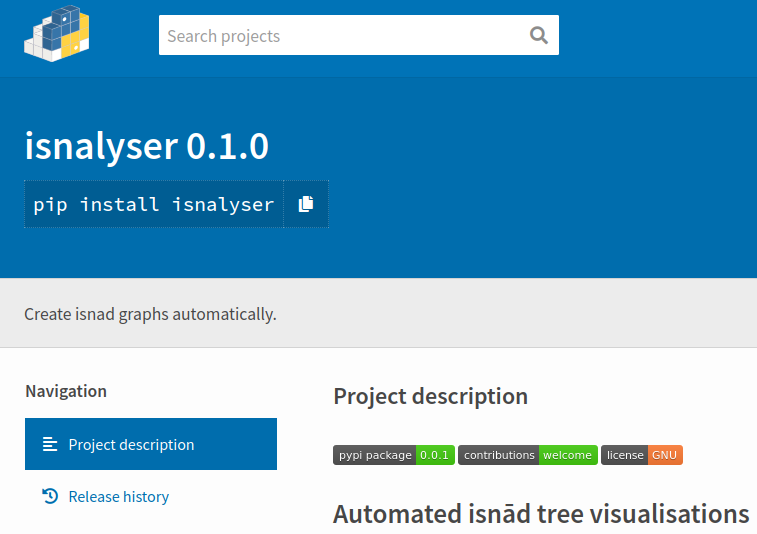
\includegraphics[width=.6\linewidth]{figures/pypi.png}
\end{figure}
\begin{itemize}%\setlength\itemsep{1.5em}
%	\item Ready for use
	\item If you are interested: Just \texttt{pip install isnalyser}
\end{itemize}
\end{frame} 



\begin{frame}
\frametitle{Isnalyserjs}
\framesubtitle{Making the isnalyser more accessible}
\begin{itemize}%\setlength\itemsep{1.5em}
	\item Python is great but requires coding knowledge
	\item Idea: create a web application
	\item Users can upload table and explore their data
\end{itemize}
\end{frame} 



\begin{frame}
\frametitle{Isnalyserjs}
\framesubtitle{Choosing the tools}
\begin{itemize}%\setlength\itemsep{1.5em}
	\item Natural choice: Javascript
	\item But with which extensions?
	\item Long phase of exploration
	\begin{itemize}
		\item D3, Dagre, Cytoscape, ...
	\end{itemize}
	\item Each with own strengths and weaknesses
	\item Realize that Graphviz is really great
	\item Solution: -> d3-graphviz
	\begin{itemize}
		\item Someone literally translated the whole graphviz into javascript
		\item This allowed us to use the graph layout power of graphviz and the visualization power of d3
	\end{itemize}
\end{itemize}
\end{frame} 

\begin{frame}
\frametitle{Isnalyserjs}
\framesubtitle{Getting to work}
\begin{itemize}%\setlength\itemsep{1.5em}
	\item Implement the functionalities from Python to Javascript
	\item Use gitflow to track features
	\begin{itemize}
		\item Main branch
		\item Each new feature as new branch
		\item If feature is finished, merge into main branch 
	\end{itemize}
	\begin{figure}
	\flushleft
	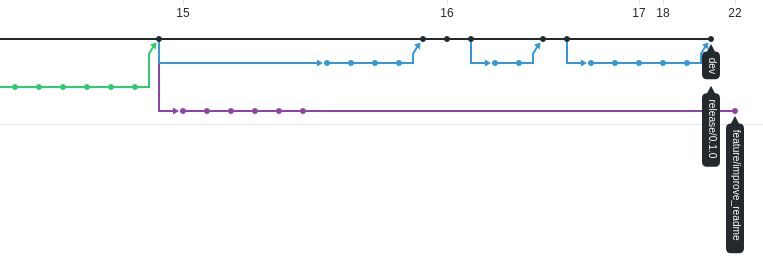
\includegraphics[width=.7\linewidth]{figures/git.png}
\end{figure}
	\item Now ready for its first release
\end{itemize}
\end{frame}



\begin{frame}
\frametitle{Isnalyserjs}
\framesubtitle{}
image here
\end{frame}




\begin{frame}
\frametitle{We want you!}
%\framesubtitle{What did we learn from this project?}
\begin{itemize}%\setlength\itemsep{1.5em}
	\item Use the tools
	\item Iteraction on different levels\\
	\begin{itemize}
		\item code
		\item github issues
		\item mail	
		\item ...
	\end{itemize}
\end{itemize}
\end{frame} 



\setbeamercolor{background canvas}{bg=orange}
\setbeamercolor{normal text}{fg=white}
\usebeamercolor[fg]{normal text}
\setbeamertemplate{itemize item}{\color{white}$\circ$}
\setbeamercolor{structure}{fg=white} % itemize, enumerate, etc
\begin{frame}
\frametitle{Conclusions}
\framesubtitle{What did we learn from this project?}
\begin{itemize}%\setlength\itemsep{1.5em}
	\item Creating a PyPI package is not that hard
	\item Git flow helps keeping track and maintaining transparency
%	\item Know your Audience
%	\item Seemingly easy problems can turn out quite hard
	\item Listen to different opinions %Alvaro v Maroussia v Stefan
	\item Most important part of the project are users
	\item Interaction happens on many levels
	\item If you interested in the two tools
	\begin{itemize}
		\item Try them out
		\item File github issues
		\item Send us mails
		\item Extent the code
	\end{itemize}
	\item Never do a live demo, so that is exactly what I'm gonna do now
\end{itemize}
\end{frame} 











